%% =========================================================================
%% Supplementary material for
%% Delegation cascades in evolutionary games: stable computation with
%% strategic depth
%% =========================================================================

\RequirePackage{float}
\documentclass[a4paper,fleqn]{cas-sc}

\usepackage[numbers,sort&compress]{natbib}
\renewcommand{\sfdefault}{lmss}
\renewcommand{\ttdefault}{lmtt}
\usepackage{placeins}
\usepackage{xr}
\externaldocument[main-]{main}

\newproof{pf}{Proof}

\definecolor{cAS}{HTML}{0072B2}
\definecolor{cCS}{HTML}{009E73}
\definecolor{cCAS}{HTML}{E69F00}
\definecolor{cAU}{HTML}{D55E00}
\definecolor{cGrey}{HTML}{4D4D4D}

\newcommand{\AS}{\textsf{AS}}
\newcommand{\CS}{\textsf{CS}}
\newcommand{\CAS}{\textsf{CAS}}
\newcommand{\AU}{\textsf{AU}}
\newcommand{\piP}{\pi_{P}}
\newcommand{\piS}{\pi_{S}}

\renewcommand{\topfraction}{0.9}
\renewcommand{\bottomfraction}{0.8}
\renewcommand{\textfraction}{0.07}
\renewcommand{\floatpagefraction}{0.75}

\begin{document}
\let\WriteBookmarks\relax
\def\floatpagepagefraction{1}
\def\textpagefraction{.001}

\shorttitle{Supplementary material: Delegation cascades}
\shortauthors{T.-K. Huynh et al.}

\title[mode=title]{Supplementary material for ``Delegation cascades in
evolutionary games: stable computation with strategic depth''}

\author[1]{Trung-Kiet Huynh}[orcid=0009-0000-5463-754X]
\author[1]{Dao-Sy Duy-Minh}[orcid=0009-0002-4501-2788]
\author[1]{Chi-Nguyen Tran}[orcid=0009-0007-6716-7269]
\author[1]{Nguyen Lam Phu Quy}[orcid=0009-0002-9694-8105]
\author[1]{Pham Phu Hoa}[orcid=0009-0001-5471-2578]

\affiliation[1]{organization={Faculty of Information Technology, University of
            Science, Vietnam National University Ho Chi Minh City},
            addressline={227 Nguyen Van Cu Street, Cho Quan Ward},
            city={Ho Chi Minh City},
            country={Vietnam}}

\begin{abstract}
This supplement contains an auxiliary proof, complete numerical-validation
results, exact result tables that duplicate graphical displays in the main
paper, additional robustness sweeps, and the standard derivation of the
fixation formula. The model, notation and equation numbers are those of the
main paper.
\end{abstract}

\maketitle

\renewcommand{\thesection}{S\arabic{section}}
\renewcommand{\thetable}{S\arabic{table}}
\renewcommand{\thefigure}{S\arabic{figure}}
\numberwithin{equation}{section}

% ===========================================================================
\section{Proof of the erosion-order lemma}
\label{supp:proof-order}

\noindent\textbf{Proof of Lemma 1.}
Write a design as a pair $(f,c)$: a first action $f$ and a flag $c$ for whether
it copies its opponent's previous action. Solving the two coupled recursions
gives the focal path in closed form in each of three cases. If the opponent
does not copy, it plays $f_{j}$ in every round whatever the focal seat does, so
a focal seat that does not copy plays $f_{i}$ throughout, and one that copies
plays $f_{i}$ in round $1$ and $f_{j}$ afterwards. If both copy then
$a_{t}=a_{t-2}$ for $t\ge3$, so the focal seat plays $f_{i}$ in odd rounds and
$f_{j}$ in even ones. In every case the path is either constant at $f_{i}$, or
equal to $f_{i}$ on a set of rounds that does not itself depend on $f_{i}$ and
to $f_{j}$ on the complement.

\AS{} plays Safe in every round and \AU{} plays Unsafe in every round, against
every opponent, so they are the pointwise smallest and largest paths in the
design set and the outer two inequalities of Eq.~\eqref{main-eq:pathwise} hold.
\CS{} and \CAS{} carry the same flag $c=1$ and differ only in $f_{i}$, which
enters each closed form monotonically, so raising $f_{i}$ from Safe to Unsafe
raises the path in some rounds and lowers it in none, which gives the middle
inequality.

For the opponent argument, fix $i$. If $i$ does not copy its path is constant
at $f_{i}$ whatever $j$ is, and the ordering holds with equality. If $i$
copies, the four opponents give the paths $(f_{i},f_{j},f_{j},\dots)$ when $j$
does not copy and $f_{i}$ on odd rounds with $f_{j}$ on even rounds when it
does. Along \AS{}, \CS{}, \CAS{}, \AU{}, the focal path is, after round $1$,
Safe throughout, Safe on the even rounds and $f_{i}$ on the odd ones, $f_{i}$
on the odd rounds and Unsafe on the even ones, and Unsafe throughout. Each path
dominates the one before it, whichever value $f_{i}$ takes.

At a fixed horizon, $m$ counts the Unsafe entries of the path and $u$ divides
that count by the horizon, so both are non-decreasing functions of the path and
inherit the two orderings. Neither depends on any other parameter of the race,
so taking the expectation over any law for $T$ preserves them. \qed

% ===========================================================================
\section{Numerical validation}
\label{supp:verification}

Table~\ref{tab:verification} reports five complementary checks: the interaction
tensor, shifted-sum arithmetic, complete stationary output, the closed form,
and the rare-mutation reduction.

% split from numerics_generated.tex; do not edit
\begin{table}[pos=t]
\centering
\caption{Verification of the scheme, in four independent checks. Block~1 compares the exact horizon expectation of Section~\ref{sec:interaction} with a Monte-Carlo estimate of the same payoff matrix: root-mean-square error over the sixteen ordered pairs and eight independent replicates, which decays at the Monte-Carlo rate $N^{-1/2}$ and which the exact route removes. Block~2 compares the stabilised evaluation of~\eqref{eq:fixation} in double precision with the same sum evaluated in $60$-digit arithmetic, worst relative error over the $n(n-1)=756$ ordered pairs of the full design space whose fixation probability is representable as a normal double. Block~3 compares the closed form with the general-purpose routine of EGTtools on the depth-zero design space, worst absolute difference over all ordered pairs. Block~4 compares the small-mutation limit with the full mutation--selection chain on a design space small enough for it ($n=3$, $Z=40$, $861$ population states).}
\label{tab:verification}
\begin{tabular*}{\tblwidth}{@{}LLR@{}}
\toprule
check & setting & discrepancy \\
\midrule
Monte Carlo vs.\ exact & $N=1\,000$ episodes & $1.080$ \\
Monte Carlo vs.\ exact & $N=10\,000$ episodes & $0.269$ \\
Monte Carlo vs.\ exact & $N=100\,000$ episodes & $0.117$ \\
Monte Carlo vs.\ exact & $N=10^{6}$ episodes & $0.034$ \\
\midrule
stabilised vs.\ $60$-digit sum & $n=28$, $Z=100$, $\beta=0.05$ & $4.4\times 10^{-16}$ \\
stabilised vs.\ $60$-digit sum & $n=28$, $Z=100$, $\beta=0.2$ & $2.8\times 10^{-16}$ \\
\midrule
closed form vs.\ EGTtools & $n=4$, $Z=50$, $\beta=0.05$ & $1.1\times 10^{-16}$ \\
closed form vs.\ EGTtools & $n=4$, $Z=50$, $\beta=0.2$ & $1.1\times 10^{-16}$ \\
closed form vs.\ EGTtools & $n=4$, $Z=100$, $\beta=0.05$ & $2.8\times 10^{-16}$ \\
closed form vs.\ EGTtools & $n=4$, $Z=100$, $\beta=0.2$ & $5.6\times 10^{-16}$ \\
closed form vs.\ EGTtools & $n=4$, $Z=200$, $\beta=0.05$ & $1.1\times 10^{-16}$ \\
closed form vs.\ EGTtools & $n=4$, $Z=200$, $\beta=0.2$ & $1.1\times 10^{-16}$ \\
\midrule
small mutation vs.\ full chain & $\mu=5\times 10^{-2}$ & $0.0910$ \\
small mutation vs.\ full chain & $\mu=2\times 10^{-2}$ & $0.0426$ \\
small mutation vs.\ full chain & $\mu=10^{-2}$ & $0.0225$ \\
small mutation vs.\ full chain & $\mu=5\times 10^{-3}$ & $0.0116$ \\
\bottomrule
\end{tabular*}
\end{table}


\paragraph{Against sampling.}
A Monte Carlo estimate of the payoff matrix converges at the expected
$N^{-1/2}$ and is still two decimal places short of the exact value at
$10^{6}$ episodes per matchup. The exact route removes that error. This matters
because the interaction index in the main paper is a difference of four
stationary regimes and would otherwise be a difference of four noisy ones.

\paragraph{Against a high-precision reference.}
This check evaluates the fixation sum in Eq.~\eqref{main-eq:fixation} in 60-digit
arithmetic and compares it with the shifted double-precision evaluation in
Eq.~\eqref{main-eq:shift}. Over the pairs whose fixation probability is representable
as a normal double, 738 of 756 at $\beta=0.05$ and 589 at $\beta=0.2$, the worst
relative errors are $4.4\times10^{-16}$ and $2.8\times10^{-16}$, respectively.
On the excluded pairs the shifted evaluation is either zero or subnormal, as
described in the main paper.

\paragraph{End-to-end stationary output.}
Against a 60-digit construction of the embedded chain, total-variation error
is $8.3\times10^{-15}$ at $\beta=0.05$ and $4.3\times10^{-16}$ at $\beta=0.2$;
the corresponding unsafe-frequency errors are below $3.5\times10^{-15}$.

\paragraph{Against an independent implementation.}
The closed form was checked against an independent implementation of the same
birth--death formula in EGTtools~\citep{domingos2023egttools} on the depth-zero
design space. The two agree to at most $5.6\times10^{-16}$ at every population
size and selection intensity tried. The systematic difference is in the other
direction: the unshifted evaluation returns exactly zero for strongly
disadvantaged mutants that Eq.~\eqref{main-eq:shift} still resolves.

\paragraph{Against the full chain.}
On a space containing the intent \AS{} at depths 0, 3 and 6, the full
mutation--selection chain has 861 population states at $Z=40$ and can be solved
directly. The error of the reduction is first order in the mutation rate: for
the joint cell the absolute difference in long-run unsafe frequency is $0.0116$
at $\mu=5\times10^{-3}$ and $0.0024$ at $\mu=10^{-3}$, an error-to-rate ratio
of 2.32 and 2.38. One Richardson step $2U(\mu/2)-U(\mu)$ on the finest pair
reproduces the small-mutation value to $2.8\times10^{-5}$.

On this reduced space the two single-mechanism cells are smaller than the
affordable finite-$\mu$ error, so they are not claimed to be individually
resolved. The interaction index is more stable because errors are largely
common-mode: it is $+0.274$ at $\mu=5\times10^{-3}$ and $+0.273$ at
$\mu=10^{-3}$, against $+0.268$ in the limit. The main paper additionally
recomputes the headline decomposition under the basin-averaged replicator
attractor, a different limit of the same game.

% ===========================================================================
\section{Complete result tables}
\label{supp:result-tables}

The exact values behind the main paper's graphical decomposition are reported
in Table~\ref{tab:decomposition}. Table~\ref{tab:regimes} compares the complete
set of attribution rules used to distinguish the rate of attribution loss from
whether attribution eventually vanishes.

%% one table per file, split from paper/tables_generated.tex by
%% paper-amc/scripts/make_amc_tables.py -- do not edit
\begin{table}[pos=t]
\centering
\caption{The two mechanisms, separately and together. Long-run Unsafe frequency $U$, mean delegation depth $\bar{d}$, declaration gap and social payoff in the stationary regime of the finite-population process. Neither mechanism does much alone; the interaction is 0.293, or 91\% of the joint effect.}
\label{tab:decomposition}
\begin{tabular}{llrrrr}
\toprule
erosion $\varepsilon$ & attribution $\phi$ & $U$ & $\bar{d}$ & gap & $\pi_S$ \\
\midrule
$0$ & $1$ & 0.0000 & 6.00 & 0.000 & 68.0 \\
$0.2$ & $1$ & 0.0176 & 1.99 & 0.358 & 58.3 \\
$0$ & $0.75$ & 0.0115 & 5.95 & 0.000 & 65.5 \\
$0.2$ & $0.75$ & 0.3225 & 6.00 & 0.738 & -0.8 \\
\midrule
\multicolumn{2}{l}{interaction} & +0.2934 & & & \\
\bottomrule
\end{tabular}
\end{table}

%% one table per file, split from paper/regimes_generated.tex by
%% paper-amc/scripts/make_amc_tables.py -- do not edit
\begin{table}[pos=t]
\centering
\caption{Attribution regimes. Long-run Unsafe frequency, mean delegation depth and social payoff when the law mapping depth to the principal's share of the harm is changed, with everything else at the baseline. The shelter survives every rule whose attribution keeps falling in the depth, including the equal split, and closes under every rule that is bounded below.}
\label{tab:regimes}
\begin{tabular}{llrrrr}
\toprule
rule & setting & $a(D)$ & $U$ & $\bar{d}$ & $\pi_S$ \\
\midrule
geometric, $\phi^{d}$ & $\phi=0.75$ & 0.178 & 0.3225 & 6.00 & -0.8 \\
strict, $1$ & -- & 1.000 & 0.0176 & 1.99 & 58.3 \\
equal split, $1/(1+d)$ & -- & 0.143 & 0.3224 & 6.00 & -0.8 \\
floored, $\max(\phi^{d}, a_{\min})$ & $a_{\min}=0.25$ & 0.250 & 0.2317 & 5.07 & 17.1 \\
floored, $\max(\phi^{d}, a_{\min})$ & $a_{\min}=0.5$ & 0.500 & 0.0633 & 2.99 & 50.0 \\
super-attribution, $\phi^{d}$ & $\phi=1.1$ & 1.772 & 0.0159 & 1.92 & 58.5 \\
super-attribution, $\phi^{d}$ & $\phi=1.25$ & 3.815 & 0.0030 & 1.21 & 60.2 \\
\bottomrule
\end{tabular}
\end{table}


% ===========================================================================
\section{Additional robustness results}
\label{supp:robustness}

Across 43 parameter cells, interaction is positive in 91\%, with median 0.294
and interquartile range $[0.243,0.299]$; per-layer attribution selects greater
depth than pass-through in every cell. Three non-positive cells are saturated
at unsafe frequency one, and the fourth uses the collapse kernel, which
suppresses delegation.

The headline level is sensitive to liability and the depth ceiling but stable
to the evolutionary-process parameters. Across
$L\in\{5,10,20,40,80\}$, the joint unsafe frequency is $0.949$, $0.323$,
$0.322$, $0.322$ and $5\times10^{-5}$; among positive-interaction cells, the
interaction share ranges from 0.001 to 1.12. At
$\bar D\in\{4,6,8\}$, the joint values are $0.136$, $0.322$ and $0.513$, with
mean depth equal to the ceiling, whereas pass-through remains at unsafe
frequency 0.018 and mean depth two. The joint value is 0.3225 for
$Z\in\{50,100,200\}$ and ranges only from 0.3168 to 0.3225 over
$\beta\in[0.01,0.2]$.

Kernel shape changes the result (Figure~\ref{fig:robustness}B). Collapse noise
reduces mean depth to 0.0002 and unsafe frequency to $2\times10^{-5}$, whereas
uniform noise raises the latter to 0.520. Two interpolating families hold the
second eigenvalue of $M$ at $1-\varepsilon$ while varying drift direction and
severity (Table~\ref{tab:kernelshape}). Their outcomes range from
$2\times10^{-5}$ to 0.520, so neither the spectral gap nor directionality
orders the result. Within these families, delegation collapses when the harm
caused by one hand-off crosses approximately $[0.51,0.61]$; the ladder instead
has $m(1)=0$, allowing depth to accumulate before its private cost appears.

\input{tab_kernelshape}

The cascade is not created by a free organisational benefit. Setting $g=0$
leaves unsafe frequency at 0.321 and mean depth at 5.98, because erosion raises
the focal race payoff from 41.3 to 48.1 across the depth range. Adding
coordination cost leaves the ceiling binding through $c=0.16$ and mean depth at
5.95 for $c=0.20$; depth falls materially only when the deepest chain's net
organisational benefit approaches zero.

\begin{figure}[pos=tb]
\centering
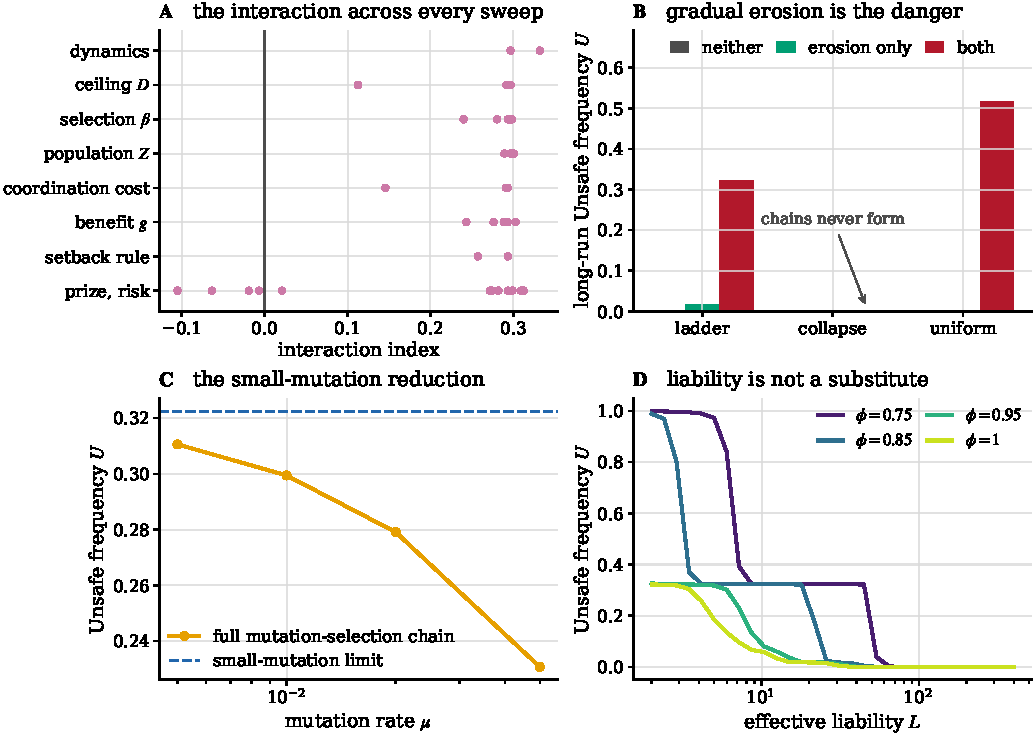
\includegraphics[width=\linewidth]{figures/fig08_robustness.pdf}
\caption{Robustness. \textbf{(A)}~The interaction index across every sweep;
each dot is one parameter cell. \textbf{(B)}~The three named drift kernels. The
\emph{ladder} produces the cascade; \emph{collapse} deters delegation
altogether; \emph{uniform} noise is worse than the graded ladder, so the effect
is not about the direction of the slippage. \textbf{(C)}~The small-mutation
limit against the full mutation--selection chain on the three-design sub-space,
over $\mu\in[0.005,0.05]$ at $Z=60$; Table~\ref{tab:verification} reports the
same check at $Z=40$ and down to $\mu=0.001$. \textbf{(D)}~Long-run unsafe
frequency against the effective liability at four attribution retentions; a
lower $\phi$ shifts the whole curve rather than tilting it, which is the
population-level counterpart of the failure-depth result in the main paper.}
\label{fig:robustness}
\end{figure}

\FloatBarrier

% ===========================================================================
\section{The stationary regime in closed form}
\label{supp:fixation}

The derivation of Eq.~\eqref{main-eq:fixation} is standard and is repeated here so
that the constants in Algorithm~\ref{main-alg:main} can be read off. In a population
of $Z$ individuals holding $k$ copies of the invader $I$ and $Z-k$ of the
resident $R$, an update picks an ordered pair of distinct individuals uniformly,
so the probability that an $R$ individual is picked to revise and an $I$
individual to imitate is $\frac{Z-k}{Z}\frac{k}{Z-1}$, and symmetrically in the
other direction. With the Fermi rule the two transition probabilities are
\begin{equation}
  T^{+}(k) = \frac{k(Z-k)}{Z(Z-1)}\,
    \frac{1}{1+e^{-\beta(\pi_{I}(k)-\pi_{R}(k))}},
  \qquad
  T^{-}(k) = \frac{k(Z-k)}{Z(Z-1)}\,
    \frac{1}{1+e^{\beta(\pi_{I}(k)-\pi_{R}(k))}}.
  \label{eq:supp-rates}
\end{equation}
Their ratio is
$T^{-}(k)/T^{+}(k)=e^{-\beta(\pi_{I}(k)-\pi_{R}(k))}$, in which the common
sampling factor cancels. The classical absorption formula for a
one-dimensional birth--death chain with absorbing boundaries at $k=0$ and
$k=Z$,
\[
  \rho_{R\to I}
  = \left[1+\sum_{m=1}^{Z-1}\prod_{k=1}^{m}
    \frac{T^{-}(k)}{T^{+}(k)}\right]^{-1},
\]
therefore gives Eq.~\eqref{main-eq:fixation} directly. Because
$\pi_{I}-\pi_{R}$ is affine in $k$, the exponent
$\theta_{m}=-\beta\sum_{k\le m}(\pi_{I}(k)-\pi_{R}(k))$ is a quadratic
polynomial in $m$ and the whole vector
$(\theta_{1},\dots,\theta_{Z-1})$ is one cumulative sum, which gives the
$O(Z)$ claim in the main paper. Two limits are useful as unit tests: at
$\beta=0$ every ratio is one and $\rho=1/Z$, and for a neutral game the same
holds at every $\beta$.

In exact arithmetic every $\rho_{i\to j}$ is strictly positive at finite
$\beta$, so the embedded chain is irreducible and its stationary distribution
is unique. Irreducibility is more than is needed and more than double precision
delivers. Uniqueness requires only one closed communicating class, so a routine
that returns exactly zero for a strongly disadvantaged mutant does not by
itself make the stationary vector ambiguous; it moves designs into transient
classes, which receive stationary mass exactly zero rather than their true
subnormal mass. At $\beta=0.2$ that happens for
$\{\CAS{}@0,\AU{}@0\}$, which is transient in double precision while the
remaining 26 designs form the unique closed class. Under the unshifted
evaluation the closed class instead shrinks to a single absorbing design, and
the stationary regime stops carrying information.

\bibliographystyle{elsarticle-num-names}
\bibliography{refs}

\end{document}
